\def\VCDate{2015/12/12}\def\VCVersion{(Current)}
\documentclass{article}
\usepackage[screen]{geometry}
\usepackage{ProofPower, graphicx,amsmath,multicol}
\setlength{\columnsep}{2cm}
\begin{document}
\title{Lab 5}
\author{Ai Nguyen}
\maketitle
Lab to explore RAID storage. Using this technique, it is possible to recover from a failed disk drive by stripping data across 3 drives and storing the xor of those 3 values into the 4th (parity) drive \\
\section{C algorithm}
\begin{GFT}{C source code written to file lab6.c}
\+\#include <stdio.h>\\
\+\#include <math.h>\\
\+\#define N 48 //Symbolic constant vs Creates memory location\\
\+char dataIn[] = "This is some test data for a RAID simulator";\\
\+char dataOut[N]; //Partial initialization of array\\
\+char disk1[N/3]; // expect to store "Tsso sdaoaA mar"\\
\+char disk2[N/3];\\
\+char disk3[N/3];\\
\+char disk4[N/3];\\
\+int main()\\
\+\{\\
\+  printf("dataIn<\%s>\Backslash{}n", dataIn);\\
\end{GFT}
\begin{multicols}{2}
Stripe the data across the drives and store parity in disk4
\begin{GFT}{C source code appended to file lab6.c}
\+  int i =0, j =0;\\
\+  for(i =0, j =0; i < N-2; i+=3, j++)\\
\+  \{	disk1[j] = dataIn[i];\\
\+	disk2[j] = dataIn[i+1];\\
\+	disk3[j] = dataIn[i+2];\\
\+	disk4[j] = disk1[j] \Circumflex{} disk2[j] \Circumflex{} disk3[j];\\
\+  \}\\
\end{GFT}
\columnbreak
\begin{GFT}{C source code appended to file lab6.c}
\+  printf("dataOut<\%s>\Backslash{}n", dataOut);\\
\+  printf("disk1<\%s>\Backslash{}n", disk1);\\
\+  printf("disk2<\%s>\Backslash{}n", disk2);\\
\+  printf("disk3<\%s>\Backslash{}n", disk3);\\
\+  printf("disk4<\%s>\Backslash{}n", disk4);\\
\end{GFT}
\end{multicols}
\clearpage
Suppose disk2 is corrupted(like politicians)
\begin{multicols}{2}
\begin{GFT}{C source code appended to file lab6.c}
\+for (i=0; i < N/3; i++)\\
\+\{\\
\+  disk2[i] = '.';\\
\+\}\\
\+for (i=0 , j =0; i < N - 2; i+=3, j++)\\
\+\{\\
\+  dataOut[i] = disk1[j];\\
\+  dataOut[i+1] = disk2[j];\\
\+  dataOut[i+2] = disk3[j];\\
\+\}\\
\+printf("dataOut<\%s>\Backslash{}n", dataOut);\\
\end{GFT}
Fix/rebuild disk2
\begin{GFT}{C source code appended to file lab6.c}
\+for (i =0; i < N/3; i++)\\
\+\{\\
\+  disk2[i] = disk1[i] \Circumflex{} disk3[i] \Circumflex{} disk4[i];\\
\+\}\\
\end{GFT}
\columnbreak
unstripe data across drives and store msg in dataOut
\begin{GFT}{C source code appended to file lab6.c}
\+for(i =0, j=0; j < N/3; i+=3, j++)\\
\+\{\\
\+  dataOut[i] = disk1[j];\\
\+  dataOut[i+1] = disk2[j];\\
\+  dataOut[i+2] = disk3[j];\\
\+\}\\
\+printf("dataOut<\%s>\Backslash{}n",dataOut);\\
\+  return 0;\\
\+\}\\
\end{GFT}
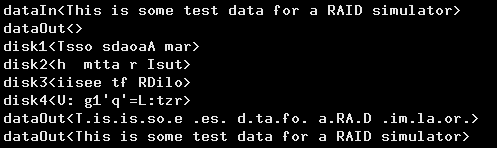
\includegraphics[scale=.5]{lab6c.png}
\end{multicols}
\clearpage\section{ASM Code}
\subsection{Main}
First we create some constants for the size of our (size of string). Use $.equ$ to assign names to numbers.
\begin{description}
\item[N]  size of $dataIn$ and $dataOut$ without counting terminated character.
\item[M]  size of $msg$
\item[M1]  size of $msg1$
\item[M2]  size of $msg2$
\item[DISK\_SIZE] size for disks
\end{description}
\begin{GFT}{asm source code written to file lab6.s}
\+.equ N,53	 \\
\+.equ M,20\\
\+.equ M1,29\\
\+.equ M2,37\\
\+.equ DISK\_SIZE, 23\\
\end{GFT}
Data section will include:
\begin{description}
\item[dataIn]  Storing test data for our program
\item[dataOut]  Storing the result from our program. Since we need $dataOut$ the same with $dataIn$, I initialized it the same with $dataIn$ to have the same size.
\item[disk1,disk2,disk3,disk4] Array for each disk. I initialized each array with their names first and all spaces following ($number of char = DISK\_SIZE$)
\item[msg,msg1,msg2, endline] These string variables is just for making the output more readable and clearer  
\end{description}
\clearpage
\begin{GFT}{asm source code appended to file lab6.s}
\+.data\\
\+  dataIn: .string "DataIn: This is some test data for a RAID simulator  "\\
\+  dataOut: .string "DataOut: This is some test data for a RAID simulator  "\\
\+  disk1: .string "Disk1:                 "\\
\+  disk2: .string "Disk2:                 "\\
\+  disk3: .string "Disk3:                 "\\
\+  disk4: .string "Disk4:                 "\\
\+  msg: .string "ASM RAID simulator\Backslash{}n"\\
\+  msg1: .string "After one disk is corrupted\Backslash{}n"\\
\+  msg2: .string "After rebuilding the corrupted disk\Backslash{}n"\\
\+  endline: .string "\Backslash{}n"\\
\end{GFT}
We won't use $printf$ from C library to print what we need but the system call technique from ASM
\begin{multicols}{2}
First print out $msg$, $dataIn$, $endline$
\begin{GFT}{asm source code appended to file lab6.s}
\+.text\\
\+.globl \_start\\
\+\_start:\\
\+\\
\+mov \$M, \%edx\\
\+mov \$msg, \%ecx\\
\+mov \$1, \%ebx\\
\+mov \$4, \%eax\\
\+int \$0x80\\
\end{GFT}
\columnbreak
\begin{GFT}{asm source code appended to file lab6.s}
\+mov \$N, \%edx\\
\+mov \$dataIn, \%ecx\\
\+mov \$1, \%ebx\\
\+mov \$4, \%eax\\
\+int \$0x80\\
\+\\
\+mov \$1, \%edx\\
\+mov \$endline, \%ecx\\
\+mov \$1, \%ebx\\
\+mov \$4, \%eax\\
\+int \$0x80\\
\end{GFT}
\end{multicols}
\clearpage
3 blocks of code above have the same syntax in the format:
\begin{itemize}
\item Copy size of buffer to $\%edx$
\item Copy address of buffer to $\%ecx$
\item Copy file descriptor to $\%ebx$. In this case, we need $1$ for STOUT
\item Copy number of system call to $\%eax$. We need $4$ for system write.
\end{itemize}
Then we call $load\_data$ to store data into disks. This function doesn't take any parameter.
\begin{GFT}{asm source code appended to file lab6.s}
\+\# store data to disks\\
\+call load\_data\\
\end{GFT}
After loading data. Print it out with the same syntax we use before for system writing. For readable output, we print $endline$ after each disk priting.
\begin{multicols}{2}
\begin{GFT}{asm source code appended to file lab6.s}
\+mov \$DISK\_SIZE, \%edx\\
\+mov \$disk1, \%ecx\\
\+mov \$1, \%ebx\\
\+mov \$4, \%eax\\
\+int \$0x80\\
\+\\
\+mov \$1, \%edx\\
\+mov \$endline, \%ecx\\
\+mov \$1, \%ebx\\
\+mov \$4, \%eax\\
\+int \$0x80\\
\end{GFT}
\columnbreak
\begin{GFT}{asm source code appended to file lab6.s}
\+mov \$DISK\_SIZE, \%edx\\
\+mov \$disk2, \%ecx\\
\+mov \$1, \%ebx\\
\+mov \$4, \%eax\\
\+int \$0x80\\
\+\\
\+mov \$1, \%edx\\
\+mov \$endline, \%ecx\\
\+mov \$1, \%ebx\\
\+mov \$4, \%eax\\
\+int \$0x80\\
\end{GFT}
\end{multicols}
\clearpage
\begin{multicols}{2}
\begin{GFT}{asm source code appended to file lab6.s}
\+mov \$DISK\_SIZE, \%edx\\
\+mov \$disk3, \%ecx\\
\+mov \$1, \%ebx\\
\+mov \$4, \%eax\\
\+int \$0x80\\
\+\\
\+mov \$1, \%edx\\
\+mov \$endline, \%ecx\\
\+mov \$1, \%ebx\\
\+mov \$4, \%eax\\
\+int \$0x80\\
\end{GFT}
\columnbreak
\begin{GFT}{asm source code appended to file lab6.s}
\+mov \$DISK\_SIZE, \%edx\\
\+mov \$disk4, \%ecx\\
\+mov \$1, \%ebx\\
\+mov \$4, \%eax\\
\+int \$0x80\\
\+\\
\+mov \$1, \%edx\\
\+mov \$endline, \%ecx\\
\+mov \$1, \%ebx\\
\+mov \$4, \%eax\\
\+int \$0x80\\
\end{GFT}
\end{multicols}
We will make one of four disks corrupt by calling function $make\_corrupt$. This function will take one parameter, which is the address of the disk we want to be corrupted (in the code, we use $\$disk2$)
\begin{multicols}{2}
\begin{GFT}{asm source code appended to file lab6.s}
\+push \$disk2 \#disk2 is corrupted\\
\+call make\_corrupt\\
\+add \$4, \%esp\\
\end{GFT}
Print dataOut when one disk is corrupted
\begin{GFT}{asm source code appended to file lab6.s}
\+mov \$M1, \%edx\\
\+mov \$msg1, \%ecx \# print msg1\\
\+mov \$1, \%ebx\\
\+mov \$4, \%eax\\
\+int \$0x80\\
\end{GFT}
\columnbreak
\begin{GFT}{asm source code appended to file lab6.s}
\+call print\_dataOut\\
\+\\
\+\# print msg2\\
\+mov \$M2, \%edx\\
\+mov \$msg2, \%ecx\\
\+mov \$1, \%ebx\\
\+mov \$4, \%eax\\
\+int \$0x80\\
\end{GFT}
\end{multicols}
\clearpage
After make one disk corrupted, we rebuild that disk by doing XOR 3 other disks. Calling funtion $rebuild$ that take 4 parameter. First 3 disks is to rebuild the corrupted one, and the fourth disk is the one needed to rebuild.
\begin{multicols}{2}
\begin{GFT}{asm source code appended to file lab6.s}
\+\#Rebuild corrupted disk\\
\+push \$disk1\\
\+push \$disk3\\
\+push \$disk4\\
\+push \$disk2	\# this for fixing\\
\+call rebuild\\
\+add \$12, \%esp\\
\end{GFT}
\columnbreak
Then print dataOut to test our program
\begin{GFT}{asm source code appended to file lab6.s}
\+call print\_dataOut\\
\+\#End \\
\+mov \$1, \%eax\\
\+mov \$0, \%ebx\\
\+int \$0x80\\
\end{GFT}
\end{multicols}
\subsection{Testing}
\begin{multicols}{2}
when disk 1 is corrupted \\ \\ \\ 
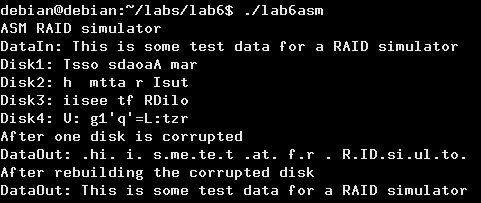
\includegraphics[scale=.5]{lab6asm1.png}
\columnbreak
\\ when disk 2 is corrupted \\ \\ \\ 
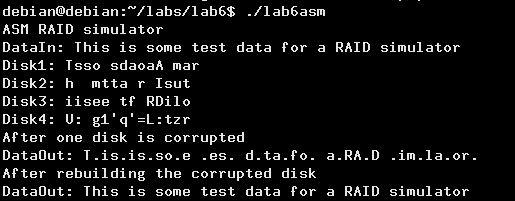
\includegraphics[scale=.5]{lab6asm2.png}
\end{multicols}
\clearpage
\subsection{load\_data}
This function is for loading data into 4 buffers (disks). For each group of 3 characters in $dataIn$ (the first group is from the beginning):
\begin{description}
\item[disk1] store $1^{st}$ letter of that group
\item[disk2] store $2^{nd}$ letter of that group
\item[disk3] store $3^{rd}$ letter of that group
\item[disk4] doing XOR of $disk1$, $disk2$ and $disk3$
\end{description}
Use $\%esi$ for $i$ (index of $dataIn$) and $\%edi$ for $j$ (index of disks). \\
Since I initialized 4 buffers (disks) in the format : "Disk1: [16 spaces]", the data read from $dataIn$ will load to each disk beginning at $8^{th}$ character, or at index $i=7$. For $dataIn$, the data we need is from index $j=8$
\begin{GFT}{asm source code appended to file lab6.s}
\+load\_data:\\
\+push \%ebp\\
\+mov \%esp, \%ebp\\
\+mov \$8, \%esi		\#i = 8\\
\+mov \$7, \%edi		\#j = 7\\
\end{GFT}
Begin of the loop ($\_L1$) The loop will stop when \( i < N - 2\). Since $N=53$, we will compare $\%esi$ with 51. If $\%esi$ is greater than 51, break the loop by jumping to $_L2$, the end of function.
\begin{GFT}{asm source code appended to file lab6.s}
\+\_L1:\\
\+cmp \$51, \%esi		\# N-2\\
\+jge \_L2			\# if i >= 51\\
\end{GFT}
\begin{multicols}{2}
Body of the loop
\begin{GFT}{asm source code appended to file lab6.s}
\+movb dataIn(\%esi), \%cl\\
\+movb \%cl, disk1(\%edi)\\
\+inc \%esi\\
\+movb dataIn(\%esi), \%cl\\
\+movb \%cl, disk2(\%edi)\\
\+inc \%esi\\
\+movb dataIn(\%esi), \%cl\\
\+movb \%cl, disk3(\%edi)\\
\+xor disk1(\%edi),\%cl\\
\+xor disk2(\%edi),\%cl\\
\+movb \%cl, disk4(\%edi)\\
\+inc \%esi\\
\+inc \%edi\\
\+jmp \_L1\\
\end{GFT}
End of the loop
\begin{GFT}{asm source code appended to file lab6.s}
\+\_L2:\\
\+mov \%ebp, \%esp\\
\+pop \%ebp\\
\+ret\\
\end{GFT}
\columnbreak
In this lab, we use \textit{indexed addressing mode} to access the data from $dataIn$ or load data to disks. The syntax will be: 
\[location(index)\]
It is similar to the syntax of array. If we need element with index $i$ in an array, we use $array[i]$; for ASM, if we want to access first character of $dataIn$ (there is no array in ASM, it is actually just a buffer), we use $dataIn(\%esi)$ with $\%esi = 0$ \\ \\
Since we move a character (8-bit or 1 byte) from $dataIn$ to each disk at a time, we use register $\%cl$ instead of $\%eax$ or $\%ebx$, which are 32-bit. $\%cl$ is first part of register $\%ecx$, and its size is only 8-bit, which is good for our purpose. Moreover, we need to use $movb$ instruction also for copying each byte at a time.
\end{multicols}
\clearpage
\subsection{make\_corrupt}
\begin{multicols}{2}
\begin{GFT}{asm source code appended to file lab6.s}
\+make\_corrupt:\\
\+push \%ebp\\
\+mov \%esp, \%ebp\\
\+mov 8(\%ebp), \%eax\\
\+mov \$0, \%edi\\
\+\_L3:\\
\+cmp \$DISK\_SIZE, \%edi\\
\+jg \_L4\\
\+movb \$'.', (\%eax,\%edi,1)\\
\+inc \%edi\\
\+jmp \_L3\\
\+\_L4:\\
\+mov \%ebp, \%esp\\
\+pop \%ebp\\
\+ret\\
\end{GFT}
\columnbreak
This function is for making the disk we want corrupted."Corrupted" in this case just simply means that we change all the characters in that disk into the character \textbf{'.'}. The function will take one parameter, which is the address of the disk need to be corrupted. \\ \\
We will need the loop for doing so. The loop begins from $\_L3$ and end at $\_L4$, with the condition $\%edi$ \textgreater $DISK\_SIZE$ to break out the loop. \\ \\
Since I create this function for making any disk corrupted, not specific one, I will not use the syntax of \textit{indexed addressing mode} I mentioned before ($disk2(\%edi)$). Instead, I use \textit{indexed indirect addressing mode}: 
\[ ( \%eax,\%edi,1) \]
which means start at $\%eax$, go $\%edi$ location forward, which each location being 1 byte big.
\end{multicols}
\clearpage
\subsection{print\_dataOut}
This function is for loading data into $dataOut$ (for result) and then print it out. We will use the same technique in function $load_data$ before. The data we need to store in $dataOut$ begins from index $i=9$. Again, the data from each disk we need to access begins from index $j=7$.
\begin{multicols}{2}
\begin{GFT}{asm source code appended to file lab6.s}
\+print\_dataOut:\\
\+push \%ebp\\
\+mov \%esp, \%ebp\\
\+mov \$9, \%esi	\# i = 9\\
\+mov \$7, \%edi	\# j = 7\\
\+\_L5:\\
\+cmp \$DISK\_SIZE, \%edi	\\
\+jge \_L6\\
\end{GFT}
Body of the loop
\begin{GFT}{asm source code appended to file lab6.s}
\+movb disk1(\%edi), \%cl	\#disk1[j]\\
\+movb \%cl, dataOut(\%esi)	\#dataOut[i]\\
\+inc \%esi\\
\+movb disk2(\%edi), \%cl	\#disk2[j]\\
\+movb \%cl, dataOut(\%esi)	\#dataOut[i+1]\\
\+inc \%esi\\
\+movb disk3(\%edi), \%cl	\#disk3[j]\\
\+movb \%cl, dataOut(\%esi)	\#dataOut[i+2]\\
\+inc \%esi\\
\+inc \%edi\\
\+jmp \_L5\\
\end{GFT}
\columnbreak
\begin{GFT}{asm source code appended to file lab6.s}
\+\_L6:\\
\end{GFT}
End of loop and print $dataOut$
\begin{GFT}{asm source code appended to file lab6.s}
\+mov \$N, \%edx\\
\+mov \$dataOut, \%ecx\\
\+mov \$1, \%ebx\\
\+mov \$4, \%eax\\
\+int \$0x80\\
\+\\
\+mov \$1, \%edx\\
\+mov \$endline, \%ecx\\
\+mov \$1, \%ebx\\
\+mov \$4, \%eax\\
\+int \$0x80\\
\+\\
\+mov \%ebp, \%esp\\
\+pop \%ebp\\
\+ret\\
\end{GFT}
\end{multicols}
\clearpage
\subsection{rebuild}
\begin{multicols}{2}
\begin{GFT}{asm source code appended to file lab6.s}
\+rebuild:\\
\+push \%ebp\\
\+mov \%esp, \%ebp\\
\+mov \$7, \%edi	\# j = 7\\
\+mov \$DISK\_SIZE, \%edx\\
\+\_L7:\\
\+cmp \$DISK\_SIZE, \%edi\\
\+jge \_L8\\
\+mov 20(\%ebp), \%eax\\
\+movb (\%eax,\%edi,1), \%cl\\
\+mov 16(\%ebp), \%eax\\
\+xor (\%eax,\%edi,1),\%cl\\
\+mov 12(\%ebp), \%eax\\
\+xor (\%eax,\%edi,1),\%cl\\
\+mov 8(\%ebp), \%eax	\#this need rebuilding\\
\+movb \%cl, (\%eax,\%edi,1)\\
\+inc \%edi\\
\+jmp \_L7\\
\+\_L8:\\
\+mov \%ebp, \%esp\\
\+pop \%ebp\\
\+ret\\
\end{GFT}
\columnbreak
This function is for fixing/rebuilding the corrupted disk from 3 other disks. \\
Since I make $make\_corrupt$ for any disk I want to be corrupted, I need to make this one also general, which means not for any specific disk. \\
First 3 parameters ($20(\%ebp)$, $16(\%ebp)$, $12(\%ebp)$) are those normal disks (order is not important), and last parameter ($8(\%ebp)$) is for the corrupted disk. \\ \\
We use the same technique with function $make\_corrupt$, using the \textit{indexed indirect addressing mode}, and of course, index $\%edi$ of each disk starts from 7. \\
The corrupted disk is fixed by doing XOR of 3 other disks.
\end{multicols}
\end{document}
